\documentclass[12pt]{article}

\usepackage{multirow}
\usepackage[utf8]{inputenc}
\usepackage{amsmath,amssymb,amsfonts,amssymb,amstext,amscd}
\usepackage[comma,numbers,sort&compress]{natbib}
\usepackage{epsfig}
\usepackage{epsf}
\usepackage{graphicx}
\usepackage{rotating}
\usepackage{textcomp}
\usepackage{latexsym}
\textwidth 160 mm 
\textheight 210 mm 
\oddsidemargin 0pt 
\evensidemargin 0pt 
\topmargin -4mm 
\headheight 0pt 
\headsep 1.25cm 
\renewcommand{\baselinestretch}{1.2} 
\newcommand{\fn}{\footnotesize}

\begin{document}

\bibliographystyle{/home/simonson/tex/misc/plos2015} 

\parindent 0mm

%\hfill \today

\vspace{5cm}

\begin{center}

\Large 
 
{\bf Computational design of PDZ domains: parameterization and performance of a simple model}
 
\vspace{1cm}

\normalsize

David Mignon$^1$, Nicolas Panel$^1$, Xingyu Chen and Thomas Simonson$^{\ast}$
 
\vspace{1cm}

$^{\dag}$Laboratoire de Biochimie (UMR CNRS 7654), Ecole Polytechnique, Palaiseau, France 
$^1$Joint first authors. $^{\ast}$Corresponding author: thomas.simonson@polytechnique.fr 

\end{center} 

\vfill

Short title: Computational design of PDZ domains 
%\\ Keywords: 

\pagebreak

\subsection*{Abstract}
PDZ domains help direct protein-protein interactions and have been extensively studied and engineered. Here, a protein design
energy function is optimized for a small set of PDZ domains. It combines a molecular mechanics protein energy, Generalized
Born solvent, and an empirical unfolded state model characterized by amino acid type-dependent chemical potentials. These are
optimized using a maximum likelihood formalism and several implementation variants. Sequences designed with the best variants
are almost all recognized by the Superfamily fold recognition tool and have similarity scores relative to experimental sequences
comparable to similarities between natural PDZ domains and to sequences designed with the Rosetta software. Three Tiam1 designs
proved stable in 200--500 ns molecular dynamics simulations. The model is then used to redesign the hydrophobic core of four
of the PDZ domains, by gradually varying a bias potential that alters the chemical potential of hydrophobic amino acid types.
The tendency of each position to retain, lose, or gain a hydrophobic character represents a novel, structure-based measure of
hydrophobicity, whose mean value differs by a factor of two between some proteins. In a second application, we redesign four
Tiam1 positions involved in peptide binding and specificity, three of which are part of the hydrophobic core. The calculations
are done for the apo protein and with two different peptide ligands. The designed sequences are homologous to the wildtype
sequence, LKLL, and an experimental quadruple mutant, MEFV, that has different affinities for the two peptides. Experimental
affinity differences between protein variants are reproduced qualitatively.

\pagebreak

\subsection*{Author summary}
Computational protein design is an emerging method that seeks to engineer new properties into proteins by mimicking the
natural mechanisms of mutation and selection. Proteins that help organize networks of interactions in cells, like PDZ
domains, are attractive targets. The space of possible sequences grows exponentially with protein size, making the problem
tremendously complex. Thus, new models and parameterizations still need to be developed and explored. Here, we parameterize
one such model, using statistical inference to choose optimal parameter values. We generate millions of theoretical sequences
using a powerful Monte Carlo exploration and we compare them to natural sequences, to determine the predictive power of the
model. Results are encouraging, so that two applications are carried out. First, we do simulations that are increasingly biased
towards hydrophobic residue types, which then invade the protein from the inside out; this gives a measure of the structure's
susceptibility to, or tolerance of hydrophobic groups. Second, we study four positions in the Tiam1 PDZ domain that help establish
specific binding of its partners, and we allow them to mutate. This provides another test of predictive power, and suggests
mutations that might alter Tiam1 specificity, a step towards cellular network engineering.

\parindent 8mm

\pagebreak

\section{Introduction}
PDZ domains (for ``postsynaptic density-95/discs large/zonula occluden s-1'') are small, globular protein domains that help establish
protein-protein interaction networks in the cell \cite{Harris01,Hung02,Tonikian08,Gfeller11,Subbaiah11,Sheperd11r}. They form specific
interactions with other, target proteins, usually by recognizing a few amino acids at the target C-terminus. Due to their biological
importance, PDZ domains and their ligands have been extensively studied and engineered, including many studies with computational
methods. Peptide ligands have been designed that modulate the activity of PDZ domains involved in various pathologies \cite{Bach12,
Roberts12,Zheng15}. Engineered PDZ domains and PDZ ligands have been used to elucidate principles of protein folding and evolution
\cite{Socolich05,Kong09,Mclaughlin12,Melero14}. In addition, these small domains with their peptidic ligands provide benchmarks
to test the computational methods themselves \cite{Reina02,Schmidt10,Smith10}.

One emerging method that has been applied to several PDZ domains is computational protein design (CPD) \cite{Kuhlman06,
Lippow07,Dai10,Feldmeier13,Tinberg13,Au16}. Starting from a 3D structural model, CPD explores a large space of sequences and
conformations to identify protein variants that have certain predefined properties, such as stability or ligand binding.
Conformational space is usually defined by a library of sidechain rotamers, which can be discrete or continuous, and by
a finite set of backbone conformations or a specific repertoire of allowed backbone deformations. The energy function
usually combines physical and empirical terms \cite{Pokala04,Samish11,Li13}. Both solvent and the unfolded protein state
are described implicitly. 

Here, we consider a simple but important class of CPD variants; we optimize selected parameters of the energy function for
a group of PDZ proteins; we test the quality of the model, and we use it for two applications. Our CPD variant is implemented
in the Proteus software \cite{Schmidt08,Simonson13b,Polydorides16}. It uses an ``MMGBSA'' energy function, which combines
a molecular mechanics protein energy with a Generalized Born + Surface Area implicit solvent treatment. The folded protein
is represented by a single, fixed, backbone conformation and a discrete sidechain rotamer library. The unfolded state energy
depends only on sequence composition, not an explicit structural model. With this CPD variant, the main adjustable model
parameters are the protein dielectric constant $\epsilon_P$, a small set of atomic surface energy coefficients $\sigma_i$, and
a collection of amino acid chemical potentials, or ``reference energies'' $E^r_t$ that each represent the contribution of a
single amino acid of type $t$ to the unfolded state energy.

We optimize the reference energies $E^r_t$ using a maximum likelihood formalism and a set of eight PDZ test proteins. For two
of the proteins, Tiam1 and Cask, we compare two sets of surface coefficients and two values of the dielectric constant. The
resulting parameter sets are tested by generating designed sequences for all eight proteins and comparing them to natural
sequences, as well as sequences generated with the Rosetta energy function and software \cite{Baker06b}. We also perform
100-500 nanosecond molecular dynamics simulations for a few designed sequences, to help assess their stability; two are stable
over 200 ns and one shows stability over 500 ns similar to the wildtype.

We then apply the optimized model to two problems. First, we do a series of Monte Carlo simulations of four of our PDZ domains
where the chemical potential of the hydrophobic amino acid types is gradually increased, artificially biasing the protein
composition. As we increase the bias, hydrophobic amino acids gradually invade the protein from the inside out, forming a
hydrophobic core that is initially smaller, then becomes larger than the natural one. The propensity of each core position
to become hydrophobic at a high or low level of bias can be seen as a structure-dependent hydrophobicity index, providing
information on the designability of the protein core. The second application consists in designing four Tiam1 positions that
are known to be involved in specific target recognition, and have been experimentally mutated so as to modify the preferred
Tiam1 target \cite{Sheperd11}, increasing its preference for the Caspr4 peptide, with respect to the syndecan-1 peptide (Sdc1).
We mutate these positions through Monte Carlo simulations of either the apo-protein or the protein in complex with either peptide
ligand. The simulations give encouraging agreement with experimental sequences and binding affinities, and suggest new variants
that could have altered specificities. 

\section{The unfolded state model}
\subsection{Maximum likelihood reference energies}
We use Monte Carlo to generate a Markov chain of states \cite{FrenkelBK3,GrimmetBK}, such that the states
are populated according to a Boltzmann distribution. One possible elementary move is a ``mutation'': we modify
the sidechain type $t$ $\rightarrow$ $t'$ at a chosen position $i$ in the folded protein, assigning a particular
rotamer $r'$ to the new sidechain. At the same time, we perform the reverse mutation in the unfolded protein,
$t'$ $\rightarrow$ $t$. For a particular sequence $S$, the unfolded state energy has the form:
\begin{equation} \label{eq:unfolded}
E^u = \sum_{i \in S} E^r(t_i).
\end{equation}
The sum is over all amino acids; $t_i$ represents the sidechain type at position $i$.  The type-dependent quantities
$E^r(t) \equiv E^r_t$ are referred to as ``reference energies''. The energy change due to a mutation has the form:
\begin{equation}  \label{eq:deltaE}
\Delta E = \Delta E^f - \Delta E^u =
\left( E^f(... t'_i,r'_i ...) - E^f(... t_i,r_i ...) \right) - \left( E^r(t'_i) - E^r(t_i) \right)
\end{equation}
where $\Delta E^f$ and $\Delta E^u$ are the energy changes in the folded and unfolded state, respectively.
The reference energies are essential parameters in the simulation model. Our goal here is to choose them empirically
so that the simulation produces amino acid frequencies that match a set of target values, for example experimental
values in the Pfam database. Specifically, we will choose them so as to maximize the probability, or likelihood of
the target sequences.

Let $S$ be a particular sequence. Its Boltzmann probability is
\begin{equation}
p(S) = \frac{1}{Z} \exp(-\beta \Delta G_S),
\end{equation}
where $\Delta G_S = G^f_S - E^u_S$ is the folding free energy of $S$, $G^f_S$ is the free energy of the folded form,
$\beta = 1/kT$ is the inverse temperature and $Z$ is a normalizing constant (the partition function). We then have
\begin{equation}
kT \ln p(S) = \sum_{i \in S} E^r(t_i)  - G^f_S - kT \ln Z = \sum_{t \in \rm aa} n_S(t) E^r_t - G^f_S - kT \ln Z,
\end{equation}
where the sum on the right is over the amino acid types and $n_S(t)$ is the number of amino acids of type $t$
within the sequence $S$.

We now consider a set ${\mathcal S}$ of $N$ target sequences $S$; we denote ${\mathcal L}$ the probability of
the entire set, which depends on the model parameters $E^r_t$; we refer to ${\mathcal L}$ as their likelihood
\cite{Kleinman06}. We have
\begin{equation}
kT \ln {\mathcal L} = \sum_S \sum_{t \in \rm aa} n_S(t) E^r_t - \sum_S G^f_S - N kT \ln Z
                    = \sum_{t \in \rm aa} N(t) E^r_t - \sum_S G^f_S - N kT \ln Z,
\end{equation}
where $N(t)$ is the number of amino acids of type $t$ in the whole dataset ${\mathcal S}$.
The normalization factor or partition function $Z$ is a sum over all possible sequences $R$:
\begin{equation}
Z = \sum_R \exp(-\beta \Delta G_R) = \sum_R \exp(-\beta \Delta G^f_R) \Pi_{t \in aa} \exp(\beta n_R(t) E^r_t)
\end{equation}
In view of maximizing ${\mathcal L}$, we consider the derivative of $Z$ with respect to one of the $E^r_t$:
\begin{equation}
\frac{ \partial Z }{ \partial E^r_t } = 
   \sum_R \beta n_R(t) \exp (-\beta \Delta G^f_R) \prod_{s \in aa} \exp(\beta n_R(s) E^r_s) 
\end{equation}
We then have
\begin{equation}
\frac{kT}{Z} \frac{ \partial Z }{ \partial E^r_t }
   = \frac{ \sum_R n_R(t) \exp(-\beta \Delta G_R) }{ \sum_R \exp(-\beta \Delta G_R) } = \langle n(t) \rangle.
\end{equation}
The quantity on the right is the Boltzmann average of the number $n(t)$ of amino acids $t$ over all possible
sequences. In practice, this is the average population of $t$ we would obtain in a long MC simulation. We note
that, as usual in statistical mechanics \cite{FowlerBK}, the derivative of $\ln Z$ with respect to one
quantity ($E^r_t$) is equal to the ensemble average of the conjugate quantity ($\beta n_S(t)$).

A necessary condition to maximize $\ln {\mathcal L}$ is that its derivatives with respect to the $E^r_t$ should
all be zero. We see that
\begin{equation}
\frac{1}{N} \frac{\partial}{\partial E^r_t} \ln {\mathcal L} = \frac{1}{N} \sum_S n_S(t) - \langle n(t) \rangle 
   = \frac{N(t)}{N} - \langle n(t) \rangle
\end{equation}
so that 
\begin{equation}  \label{eq:optimum}
{\mathcal L} \hspace*{2mm} {\rm maximum} \Longrightarrow \frac{N(t)}{N} = \langle n(t) \rangle, 
\hspace*{2mm} \forall t \in {\rm aa}
\end{equation}
Thus, to maximize ${\mathcal L}$, we should choose $\{E^r_t\}$ such that a long simulation gives the same
amino acid frequencies as the target database.

\subsection{Searching for the maximum likelihood}
To approach the maximum likelihood $\{E^r_t\}$ values, starting from a current guess $\{E^r_t(n)\}$, we will
use two methods. With the first method, we  step along the gradient of $\ln {\mathcal L}$, using the update
rule \cite{Kleinman06}:
\begin{equation} \label{eq:linear}
E^r_t (n+1) = E^r_t (n) + \alpha \frac{\partial}{\partial E^r_t} \ln {\mathcal L}
= E^r_t (n) + \delta E \, ( n_t^{\rm exp} - \langle n(t) \rangle_n)
\end{equation}
Here, $\alpha$ is a constant; $n_t^{\rm exp}$ = $N(t)/N$ is the mean population of amino acid type $t$ in the target
database; $\langle \rangle_n$ indicates an average over a simulation done using the current reference energies
$\{E^r_t(n)\}$, and $\delta E$ is an empirical constant with the dimension of an energy, referred to as the update
amplitude. This update procedure is repeated until convergence. We refer to this method as the linear update method.

The second method, used previously \cite{Schmidt08,Simonson13b}, employs a logarithmic update rule:
\begin{equation} \label{eq:log}
E^r_t (n+1) = E^r_t (n) + kT \, \ln \frac{\langle n(t) \rangle_n}{n_t^{\rm exp}}
\end{equation}
where $kT$ is a thermal energy, set empirically to 0.5 kcal/mol (1 cal = 4.184 J). We refer to this as the logarithmic
update method. Both the linear and logarithmic update methods converge to the same optimum, specified by (Eq.\
\ref{eq:optimum}). 

In the later iterations, some $E^r_t$ values tended to converge slowly, with an oscillatory behavior. Therefore,
we sometimes used a modified update rule, where the $E^r_t (n+1) - E^r_t (n)$ value computed with the linear or
logarithmic method for iteration $n$ was mixed with the value computed at the previous iteration, with the
($n-1$) value having a weight of 1/3 and the current value a weight of 2/3. At each iteration, we typically ran
500 million steps (per replica) of Replica Exchange Monte Carlo.

\section{Computational methods}
\subsection{Effective energy function for the folded state}
The energy matrix was computed with the following effective energy function for the folded state:
\begin{equation} \label{eq:energy}
E = E_{\rm bonds} + E_{\rm angles} + E_{\rm dihe} + E_{\rm impr} + E_{\rm vdw} + E_{\rm Coul} + E_{\rm solv}
\end{equation}
The first six terms in (\ref{eq:energy}) represent the protein internal energy. They were taken from the
Amber ff99SB empirical energy function \cite{Cornell95}, slightly modified for CPD (see below). The last
term on the right, $E_{\rm solv}$, represents the contribution of solvent. We used a ``Generalized Born +
Surface Area'', or GBSA implicit solvent model \cite{Hawkins95}:
\begin{equation} \label{eq:casa}
E_{\rm solv} = E_{\rm GB} + E_{\rm surf} = 
\frac{1}{2} \left(\frac{1}{\epsilon_W} - \frac{1}{\epsilon_P}\right) 
   \sum_{ij} q_i q_j \left( r_{ij}^2 + b_i b_j \exp[-r_{ij}^2/4 b_i b_j] \right)^{-1/2}
   + \sum_i \sigma_i A_i
\end{equation}
Here, $\epsilon_W$, $\epsilon_P$ are the solvent and protein dielectric constants; $r_{ij}$ is the distance
between atoms $i,j$ and $b_i$ is the ``solvation radius'' of atom $i$ \cite{Hawkins95,Lopes07}. $A_i$ is
the exposed solvent accessible surface area of atom i; $\sigma_i$ is a parameter that reflects each atom's
preference to be exposed or hidden from solvent. The solute atoms were divided into 4 groups with specific
$\sigma_i$ values (see below): unpolar, aromatic, polar, and ionic. Hydrogen atoms were assigned a surface
coefficient of 0. Surface areas were computed by the Lee and Richards algorithm \cite{Lee71}, implemented
in the XPLOR program \cite{Xplor}, using a 1.5 {\AA} probe radius. Most of the MC simulations used a protein
dielectric of $\epsilon_P$ = 4 or 8 (see Results).

In the GB energy term, the atomic solvation radius $b_i$ approximates the distance from $i$ to the protein
surface and is a function of the coordinates of all the protein atoms. The particular $b_i$ form corresponds
to a GB variant we call GB/HCT, after its original authors \cite{Hawkins95}, with model parameters optimized
for use with the Amber force field \cite{Lopes07}. Since $b_i$ depends on the coordinates of all the solute
atoms \cite{Hawkins95}, an additional approximation is needed to make the GB energy term pairwise additive
and define the energy matrix. We use a ``Native Environment Approximation'', or NEA, where the solvation radius
$b_i$ of each particular group (backbone, sidechain or ligand) is computed ahead of time, with the rest of the
system having its native sequence and conformation \cite{Simonson13b,Gaillard14}.

The surface energy contribution $E_{\rm surf}$ is not pairwise additive either, because in a protein structure,
surface area buried by one sidechain may also be buried by another. To make this energy pairwise, Street et al
proposed a simple procedure \cite{Street98}. The buried surface of a sidechain is computed by summing over the
neighboring sidechain and backbone groups. For each neighboring group, the contact area with the sidechain of
interest is computed, independently of other surrounding groups. The contact areas are then summed. To avoid
overcounting of buried surface area, a scaling factor is applied to the contact areas involving buried sidechains.
Previous work showed that a scaling factor of 0.65 works well \cite{Lopes07,Gaillard14}.

The Amber force field ff99SB is slightly modified for CPD, with the original backbone charges replaced by a unified
set, obtained by averaging over all amino acid types and adjusting slightly to make the backbone portion of each
amino acid neutral \cite{Aleksandrov10b}. 

\subsection{Reference energies in the unfolded state}
In the unfolded state, the energy depends on the sequence composition through a set of reference energies $E^r_t$
(Eq.\ \ref{eq:unfolded}). The values are assigned based on amino acid types $t$, taking into account also the position
of each amino acid in the folded structure, through its buried or solvent-exposed character. Thus, for a given type
(Ala, say), there are two distinct $E^r_t$ values: a buried and an exposed value. This is done even though the reference
energies are used to represent the unfolded, not the folded state. There are three rationales for this. First, we assume
residual structure is present in the unfolded state, so that amino acids partly retain their buried/exposed character.
Second, we hypothesize that the unfolded state model compensates in a systematic way for errors in the folded state energy
function, so that the folded structure matters. Third, this strategy makes the model less sensitive to variations in
the length of surface loops, and to the proportion of surface vs.\ buried residues, which can vary widely among homologs
(see below); as a result, the model should be more transferable within a protein family.

Distinguishing buried/exposed positions doubles the number of adjustable $E^r_t$ parameters. Conversely, to reduce the
number of adjustable parameters, we group amino acids into homologous classes (given in Results). Within each class
$c$, and for each type of position (buried or exposed), the reference energies have the form
\begin{equation}
E^r_t = E^r_c + \delta E^r_t
\end{equation}
Here, $E^r_c$ is an adjustable parameter while $\delta E^r_t$ is a constant, computed as the molecular mechanics energy
difference between amino acid types within the class $c$, assuming an unfolded conformation where each amino acid interacts
only with itself and with solvent. During likelihood maximization, $E^r_c$ is optimized while $\delta E^r_t$ is held fixed.
To optimize the $E^r_c$ values, we apply the linear or logarithmic method above; the target frequencies correspond to the
experimental frequencies of the amino acid classes, $n_c^{\rm exp}$, rather than of the individual types ($n_t^{\rm exp}$, above).

\subsection{Experimental sequences}
We considered a set of eight PDZ domains, whose PDB codes are listed in Table \ref{tab:PDZ}. To define the target amino
acid frequencies for likelihood maximization, we collected homologous sequences for each of the eight. We started by a Blast
search of the Uniprot database with the PDB sequence as the query, using the Blosum62 matrix, and retained homologs with a
sequence identity, relative to the query, above a certain threshold, around 60--80\% depending on the test protein. 
Sequences that were over 95\% or 85\% identical to the query were removed, and homologs with mutual identities above 95\%
were pruned, keeping just one of the redundant variants. This led to about 40--120 homologs per test protein; see details
in Table \ref{tab:PDZ}. For each set, amino acid frequencies were computed, distinguishing buried and exposed positions.
Buried positions were defined to have a solvent-accessible surface area below 20\% of that obtained for the amino acid alone,
which led to similar numbers of buried/exposed positions. The eight sets of mean frequencies were themselves averaged, giving
the overall target amino acid frequencies (see below).
\begin{table}[h]                            
\caption{Test proteins and their homologs} \label{tab:PDZ}                      
\begin{center} 
\begin{tabular}{ccccccc} \hline \hline  
PDB  & residue & \# active & number of & E-value   & identity & protein \\
code & numbers & positions & homologs  & threshold & \% range & acronym \\ \hline
1G9O & 9-99    & 76        & 62        & 1e-32     & 67-95    & NHERF   \\
1IHJ & 12-105  & 82        & 42        & 1e-10     & 38-95    & INAD    \\
1N7E & 667-761 & 79        & 48        & 1e-45     & 84-95    & GRIP    \\
1R6J & 192-273 & 72        & 85        & 1e-43     & 85-95    & syntenin \\
2BYG & 186-282 & 82        & 43        & 1e-41     & 78-95    & DLG2    \\
3K82 & 305-402 & 80        & 50        & 1e-46     & 81-95    & PSD95   \\
1KWA & 487-568 & 74        & 126       & 7e-28     & 60-85    & Cask    \\
4GVD & 837-930 & 84        & 50        & 2e-23     & 60-85    & Tiam1   \\ \hline
\end{tabular}
\end{center}
{\small \noindent E-values are for the Blast search for experimental homologs. Identity \% is between the
homologs and the query protein. Active positions are those that can mutate during the design simulations.
}
\end{table}

\subsection{Structural models}
Structures were prepared and energy matrices computed using procedures described previously \cite{Schmidt09,Schmidt10}.
For Tiam1, two missing segments (residues 851-854 and 868-869) were built using the Modeller program \cite{Eswar06}.
In the energy matrix calculations, for each residue pair, interaction energies were computed after 15 steps of energy
minimization, with the backbone fixed and only the interactions of the pair with each other and the backbone included.
This short minimization of pairs alleviates the discrete rotamer approximation. Sidechain rotamers were described by a
slightly expanded version of the library of Tuffery et al \cite{Tuffery91}, which has a total of 254 rotamers (sum over
all amino acid types). The expansion consists in allowing additional hydrogen orientations for OH and SH groups
\cite{Gaillard14}. This rotamer library was chosen for its simplicity and because it gives very good performance in
sidechain placement tests, comparable to the specialized Scwrl4 program (which uses a much larger library) \cite{Krivov09,
Gaillard16}. 

\subsection{Monte Carlo simulations}
The Monte Carlo simulations used one- and two-position moves, where either rotamers, types, or both are changed. For two-position
moves, the second position is selected among those that have a significant (unsigned) interaction energy with the first one,
meaning that there is at least one rotamer conformation where their interaction is 10 kcal/mol or more. In addition, we mostly
perform Replica Exchange Monte Carlo (REMC), where several simulations (``replicas'' or ``walkers'') are propagated in parallel,
at different temperatures; periodic swaps are attempted between the conformations of two walkers $i$, $j$ (adjacent in temperature).
The swap is accepted with probability
\begin{equation} \label{eq:remc}
acc({\rm swap}_{ij}) = {\rm Min} \left[ 1, e^{(\beta_i - \beta_j)(\Delta E_i - \Delta E_j)} \right]
\end{equation}
where $\beta_i$, $\beta_j$ are the inverse temperatures of the two walkers and $\Delta E_i$, $\Delta E_j$ are the changes in
their folding energies due to the conformation change \cite{Kofke02,Earl05}. We use eight walkers, with thermal energies $kT_i$
that range from 0.125 to 3 kcal/mol, and are spaced in a geometric progression: $T_{i+1}/T_i$ = constant \cite{Kofke02}.
Simulations are done with the proteus program \cite{Simonson13b}; REMC uses an efficient, shared-memory, OpenMP parallelization
\cite{Mignon16}.

For the Tiam1 protein, a few simulations were also done that included a biasing potential, which penalizes sequences with
a low similarity to a reference, experimental set. The bias energy had the form
\begin{equation} \label{eq:bias}
\delta E_{\rm bias} = c \sum_i \left( S(t_i) - S_i^{\rm rand} \right),
\end{equation}
where the sum is over the amino acid positions $i$, $t_i$ is the sidechain type at position $i$, $S(t_i)$ is the (dimensionless)
Blosum40 similarity score versus the corresponding position in the Pfam RP55 sequence alignment; $S_i^{\rm rand}$ is the mean score
(versus the same Pfam column) for a random type (where all types are equiprobable), and $c$ = 0.5 kcal/mol.

\subsection{Rosetta sequence generation}
Monte Carlo simulations were also done using the Rosetta program and energy function \cite{Baker06b}. The simulations
were done using version 2015.38.58158 of Rosetta (freely available online), using the command \small
\begin{verbatim}
fixbb -s Tiam1.pdb -resfile Tiam1.res -nstruct 10000 -ex1 -ex2 -linmem_ig 10
\end{verbatim} \normalsize
where the last option corresponds to on-the-fly energy calculation, ex1 and ex2 activate an enhanced rotamer search for buried
sidechains, and default parameters are used otherwise. Simulations were run for each protein until 10000 unique low energy
sequences were identified, corresponding to run times of about 5 minutes per sequence on a single core of a recent Intel processor,
for a total of 10 hours (per protein) using 80 cores. This is comparable to the cost of the Proteus calculations (energy matrix
plus Monte Carlo).

\subsection{Sequence characterization}
Designed sequences were compared to the Pfam alignment for the PDZ family, using the Blosum40 scoring matrix and a
gap penalty of -6. Each Pfam sequence was also compared to the Pfam alignment. For these Pfam/Pfam comparisons, if a
test protein T was part of the Pfam alignment, the T/T self comparison was left out, to be more consistent with the
designed/Pfam comparisons. The Pfam alignment was the ``RP55'' alignment, with 12255 sequences. Similarities were
computed for 14 core residues and 16 surface residues, defined by their near-complete burial or exposure (listed in 
Results) and for the entire protein.

Designed sequences were submitted to the Superfamily library of Hidden Markov Models \cite{Gough01,Wilson07},
which attempts to classify sequences according to the SCOP classification \cite{Andreeva04}. Classification was
based on SCOP version 1.75 and version 3.5 of the Superfamily tools. Superfamily executes the hmmscan program,
which implements a Hidden Markov model for each SCOP family and superfamily; here hmmscan was executed with an
E-value threshold of 10$^{-10}$, using a total of 15438 models to represent the SCOP database.

To compare the diversity in the designed sequences with the diversity in natural sequences, we used a standard,
position-dependent sequence entropy \cite{DurbinBK}, computed as follows:
\begin{equation} \label{eq:entropy}
S_i = - \sum_{j=1}^6 f_j (i) \ln f_j (i)
\end{equation}
where $f_j(i)$ is the frequency of residue type $j$ at position $i$, either in the designed sequences or in the
natural sequences (organized into a multiple alignment). Instead of the usual, 20 amino acid types, we employ
six residue classes, corresponding to the following groups: \{LVIMC\}, \{FYW\}, \{G\}, \{ASTP\}, \{EDNQ\}, and
\{KRH\}. This classification was obtained by a cluster analysis of the BLOSUM62 matrix \cite{Murphy02}, and also
by analyzing residue-residue contact energies in proteins \cite{Launay07}. To get a sense of how many amino acid
types appear at a specific position $i$, we report the residue entropy in its exponentiated form, $\exp(S_i)$
(which ranges from 1 to 6), averaged over the protein chain (i.e., $S_i$ is exponentiated first, then averaged
over positions).

\subsection{Molecular dynamics simulations}
For wildtype Tiam1 and a few designed sequences, we ran MD simulations with explicit solvent. Starting structures were
taken from the MC trajectory or the crystal structure (wildtype protein) and slightly minimized with harmonic restraints
to maintain the backbone geometry. The protein was immersed in a large box of water; waters overlapping protein were
eliminated, and the solvated system was truncated to the shape of a truncated octahedral box using the Charmm graphical
interface or GUI \cite{Jo08}; the minimum distance between protein atoms and the box was 15 {\AA}; final models included
about 11000 water molecules. A few sodium or chloride ions were included to ensure overall electroneutrality. Protonation
states of histidines were assigned to be neutral, based on visual inspection. MD was done at room temperature and pressure,
using a Nose-Hoover thermostat and barostat. Long-range electrostatic interactions were treated with a Particle Mesh Ewald
approach \cite{DardenBK}. The Amber ff99SB forcefield was used for the protein; the TIP3P model \cite{Jorgensen83} was
used for water. Simulations were run for 100--500 nanoseconds, depending on the sequence, using the Charmm and NAMD programs
\cite{Brooks09,NAMD}.

\section{Results}
\subsection{Experimental structures and sequences}
We begin by a brief overview of the test proteins. 3D structures are shown in Fig.\ \ref{fig:chain3D}A; for clarity, only
four of the eight proteins are shown. 14 core residues (highlighted by their C$_{\beta}$ atoms, shown as spheres) superimpose
well between structures; loops and chain termini display large deviations, and the Tiam1 $\alpha_2$ helix is rotated slightly
outwards compared to the other three structures. Fig.\ \ref{fig:chain3D}B illustrates the similarity between all eight domains,
measured by the rms deviation between structurally-aligned C$_{\alpha}$ atoms. Structure pairs with rms deviations of 1 {\AA}
or less and 60 aligned residues or more are linked; 2BYG (DLG2) forms the center of the group, with five links; Cask is not
quite linked to 1IHJ (rms deviation of 1.3 {\AA} over 63 residues) and Tiam1 is isolated. Sequence identities are also shown,
including those between Tiam1 and its closest homologs. Overall, six proteins form a tight group, with deviations of 1 {\AA}
or less, while Cask and Tiam1 are further away. The Tiam1/Cask sequence identity is 33\%; their structural deviation is 1.7
{\AA} based on a 42-residue alignment. 
\begin{center} $\star \star \star$ insert Figure \ref{fig:chain3D} near here $\star \star \star$ \end{center}


Sequence conservation within our eight proteins and a subset of the Pfam seed alignment (half) is shown in Fig.\ \ref{fig:align}.
The 14 positions we use to define the hydrophobic core are highly, though not totally conserved within the Pfam seed alignment.
Arg, Lys and Gln appear at some of the positions, since in a small PDZ protein, the long hydrophobic portion of these sidechains
can be buried in the core while still allowing the polar tip of the sidechain to be exposed to solvent. Small amounts of Asp, and
Glu also appear, in places where the sequence alignment may not reflect closely the 3D sidechain superposition (or lack thereof).
\begin{center} $\star \star \star$ insert Figure \ref{fig:align} near here $\star \star \star$ \end{center}

\subsection{Optimizing the unfolded state model}
We optimized the reference energies $E^r_t$ for six of the eight proteins, with the other two (Tiam1, Cask) left for cross
validation. The protein dielectric constant was $\epsilon_P$ = 8, and a first set of atomic surface coefficients was used.
We refer to the resulting model either as model A or as the ($\epsilon_P$=8, S1, $n$=6) model (S1 for ``set 1''; $n$=6
represents the number of proteins used to define the target amino acid frequencies). We repeated the optimization for Tiam1
and Cask alone, to see what improvement is obtained, if any, when a smaller set of proteins is specifically optimized.
The resulting model is called A' or ($\epsilon_P$=8, S1, $n$=2). Finally, we repeated the $E^r_t$ optimization using a
second set of surface coefficients and an $\epsilon_P$ of either 8 or 4; these calculations were done for Tiam1 and Cask
alone, due to the cost of repeated optimizations with multiple proteins. The corresponding models are called B ($\epsilon_P$=8,
S2, $n$=2) and B' ($\epsilon_P$=4, S2, $n$=2). Model names are listed in Table \ref{tab:models}. The optimizations all
converged to within 0.05 kcal/mol after about 20 iterations for most amino acid types, and within 0.1 kcal/mol for the
others (the weakly-populated types), using either the linear or the logarithmic method. Table \ref{tab:Eref} indicates
the final reference energies for models A and B, which give the best performance (see below), and for model A' (closely
related to A). The $E^r_t$ values are compared to, and agree qualitatively with the energies computed from an extended
peptide structure, which provides a less empirical model of the unfolded state. Table \ref{tab:freqs} compares the amino
acid frequencies from experiment and the simulations. The theoretical populations of the different amino acid classes agree
well with experiment, with rms deviations of about 1\% for models A, A', and B, for both exposed and buried classes. The
agreement for the amino acid types is less good, with rms deviations of 3.9\%/2.4\% for model B (buried/exposed positions,
respectively) and 2.0\%/2.5\% for model A. The intra-class frequency distributions depend explicitly on the energy offsets
$\delta E^r_t$ defined within each class, which are computed with molecular mechanics (see Methods). Notice also that since
model A uses three times more target proteins than model B ($n$=6 vs.\ $n$=2), the taret frequencies are presumably defined
about $\sqrt{3}$ $\approx$ 1.7 times less precisely for model B, so a larger deviation is acceptable in principle.
\begin{table}[h]                            
\caption{Model variants} \label{tab:models}                      
\begin{center} 
\begin{tabular}{cccccl} \hline \hline  
model & model            & dielectric & $\sigma_i$ & \# target & $\sigma_i$ values (cal/mol/\AA$^2$) \\
name  & symbol           & constant   &  set       & proteins  & $^b$(unpol,arom,polar,ionic) \\ \hline
A     & ($\epsilon_P$=8,S1,$n$=6$^a$) & 8 & set 1      & 6         & -5, -12, -8, -9   \\ 
A'    & ($\epsilon_P$=8,S1,$n$=2) & 8 & set 1      & 2         & -5, -12, -8, -9   \\ 
B     & ($\epsilon_P$=8,S2,$n$=2) & 8 & set 2      & 2         & -5,-40,-80,-100   \\
B'    & ($\epsilon_P$=4,S2,$n$=2) & 4 & set 2      & 2         & -5,-40,-80,-100   \\ \hline
\end{tabular} \\
{\footnotesize $^a$Number of proteins whose composition forms the target set; $^b$atom surface energy coefficients.}
\end{center}
\end{table}

\begin{table}[h]
\caption{Unfolded state reference energies $E_t^r$ (kcal/mol)}
\label{tab:Eref}                      
\begin{center}
\small
\begin{tabular}{cccccccc} \hline \hline
    &        & \multicolumn{2}{c}{\hrulefill Model A' \hrulefill} & \multicolumn{2}{c}{\hrulefill Model A \hrulefill} &
               \multicolumn{2}{c}{\hrulefill Model B \hrulefill} \\
Residues&Peptide$^b$& Buried & Exposed & Buried & Exposed & Buried & Exposed \\ \hline
ALA     &   0.00 &   0.00 &   0.00 &   0.00 &   0.00  &   0.00 &   0.00 \\
CYS     &  -1.04 &  -1.04 &  -1.04 &  -1.04 &  -1.04  &  -0.85 &  -0.85 \\
THR     &  -3.82 &  -3.82 &  -3.82 &  -3.82 &  -3.82  &  -5.44 &  -5.44 \\
SER     &  -2.85 &  -2.71 &  -2.62 &  -3.73 &  -2.80  &  -3.71 &  -4.74 \\
ASP     &  -9.17 & -10.32 & -10.24 &  -9.19 &  -9.80  & -11.90 & -15.88 \\
GLU     &  -7.88 &  -9.03 &  -8.95 &  -7.90 &  -8.51  & -11.97 & -15.95 \\
ASN     &  -5.64 &  -6.26 &  -5.69 &  -5.94 &  -6.00  &  -7.82 & -10.22 \\
GLN     &  -4.42 &  -5.04 &  -4.46 &  -4.72 &  -4.78  &  -7.07 &  -9.47 \\
$^a$HIS$^+$ &  15.72 &  14.82 &  15.18 &  14.53 &  14.96  &  12.53 &   9.73 \\
$^a$HIS$_{\epsilon}$ &  12.62 &  11.72 &  12.08 &  11.43 &  11.85  &  10.49 & 7.69 \\
$^a$HIS$_{\delta}$ &  13.16 &  12.25 &  12.62 &  11.96 &  12.39  &  10.86 &   8.06 \\
ARG     & -25.30 & -25.97 & -24.76 & -28.29 & -28.90  & -32.00 & -35.18 \\
LYS     &  -4.21 &  -3.16 &  -2.96 &  -4.56 &  -4.47  &  -6.76 & -10.17 \\
ILE     &   1.63 &   3.12 &   2.05 &   4.72 &   2.11  &   4.63 &   3.63 \\
VAL     &  -2.25 &  -0.76 &  -1.83 &   0.83 &  -1.77  &   0.26 &  -0.74 \\
LEU     &  -1.92 &  -0.42 &  -1.49 &   1.17 &  -1.44  &  -0.12 &  -1.12 \\
MET     &  -2.44 &  -2.85 &  -3.03 &  -2.78 &  -3.54  &  -2.05 &  -2.40 \\
PHE     &  -1.42 &  -1.71 &  -3.25 &  -0.37 &  -2.55  &  -0.23 &  -4.17 \\
TRP     &  -2.66 &  -2.95 &  -4.49 &  -1.61 &  -3.79  &  -2.21 &  -6.15 \\
TYR     &  -4.56 &  -4.67 &  -5.58 &  -4.20 &  -6.10  &  -5.80 &  -9.82 \\ \hline
\end{tabular}
\end{center}
{\footnotesize \noindent $^a$His protonation states. $^b$Energies within an extended peptide structure (averaged over positions).
}
\end{table}

\begin{table}
\caption{Amino acid composition (\%) of experimental and designed PDZ proteins} \label{tab:freqs}
\hspace*{-1.5cm}
\small
\begin{tabular}{c|clcl|clcl|clcl|clcl} \hline \hline
\multirow{2}{*}{R} & \multicolumn{4}{c|}{Design, model A}& \multicolumn{4}{c|}{Experiment, n=6 set}& \multicolumn{4}{c|}{Experiment, n=2 set}
 & \multicolumn{4}{c}{Design, model B} \\
 & \multicolumn{2}{c}{Buried} & \multicolumn{2}{c|}{Exposed} & \multicolumn{2}{c}{Buried} & \multicolumn{2}{c|}{Exposed} 
 & \multicolumn{2}{c}{Buried} 
 & \multicolumn{2}{c|}{Exposed} & \multicolumn{2}{c}{Buried} & \multicolumn{2}{c}{Exposed} \\ \hline
A & 11.1 & \multirow{2}{*}{17.0} & 4.4 & \multirow{2}{*}{12.0} & 10.9 & \multirow{3}{*}{16.9} & 4.6 & \multirow{3}{*}{13.4} & 5.9 & \multirow{3}{*}{11.2} 
    & 4.6 & \multirow{3}{*}{13.4} & 4.1 & \multirow{2}{*}{12.7} & 7.2 & \multirow{2}{*}{13.6}\\
C & 0.0 & \multirow{2}{*}{[0.1]} & 0.3 & \multirow{2}{*}{[-1.4]} & 1.3 & & 0.5 & & 1.5 & & 1.2 & & 8.6 & \multirow{2}{*}{[1.5]} & 5.8 & \multirow{2}{*}{[0.2]}\\
T & 5.9 & & 7.3 & & 4.7 & & 8.3 & & 3.8 & & 7.6 & & 0.0 & & 0.6 & \\
\hline
\multirow{2}{*}{S}  & \multirow{2}{*}{4.3} & 4.3 & \multirow{2}{*}{8.7} & 8.7 & \multirow{2}{*}{5.3} & \multirow{2}{*}{5.3} & \multirow{2}{*}{7.6} & \multirow{2}{*}{7.6} & \multirow{2}{*}{4.7} & \multirow{2}{*}{4.7} & \multirow{2}{*}{10.2} & \multirow{2}{*}{10.2} & \multirow{2}{*}{4.9} & 4.9 & \multirow{2}{*}{10.7} & 10.7\\
 &  & [-1.0] &  & [1.1] &  &  &  &  &  &  &  &  &  & [0.2] &  & [0.5]\\
\hline
D & 4.5 & \multirow{1}{*}{6.7} & 5.6 & \multirow{1}{*}{16.7} & 4.3 & \multirow{2}{*}{6.8} & 6.0 & \multirow{2}{*}{17.9} & 3.5 & \multirow{2}{*}{9.6} & 6.2 
    & \multirow{2}{*}{16.7} & 7.4 & \multirow{1}{*}{9.4} & 8.0 & \multirow{1}{*}{16.1}\\
E & 2.2 & [-0.1] & 11.1 & [-1.2] & 2.5 & & 11.9 & & 6.1 & & 10.5 & & 2.0 & [-0.2] & 8.1 & [-0.6]\\
\hline
N & 2.5 & \multirow{1}{*}{4.7} & 7.5 & \multirow{1}{*}{14.0} & 2.6 & \multirow{2}{*}{4.7} & 6.7 & \multirow{2}{*}{12.2} & 1.9 & \multirow{2}{*}{2.7} & 7.4 
    & \multirow{2}{*}{16.1} & 1.8 & \multirow{1}{*}{2.8} & 8.6 & \multirow{1}{*}{17.1}\\
Q & 2.2 & [0.0] & 6.5 & [1.8] & 2.1 & & 5.5 & & 0.8 & & 8.7 & & 1.0 & [0.1] & 8.5 & [1.0]\\
\hline
H$^+$ & 1.0 & \multirow{2}{*}{1.1} & 5.2 & \multirow{2}{*}{5.6} & 1.2 & \multirow{3}{*}{1.2} & 5.0 & \multirow{3}{*}{5.0} & 0.7 & \multirow{3}{*}{0.7} & 4.7 
    & \multirow{3}{*}{4.7} & 0.1 & \multirow{2}{*}{0.9} & 1.8 & \multirow{2}{*}{4.5}\\
H$_{\epsilon}$ & 0.1 & \multirow{2}{*}{[-0.1]} & 0.4 & \multirow{2}{*}{[0.6]} & 0.0 & & 0.0 & & 0.0 & & 0.0 & & 0.6 & \multirow{2}{*}{[0.2]} & 2.2 & \multirow{2}{*}{[-0.2]}\\
H$_{\delta}$ & 0.0 & & 0.0 & & 0.0 & & 0.0 & & 0.0 & & 0.0 & & 0.2 & & 0.5 & \\
\hline
I & 16.9 & \multirow{2}{*}{52.1} & 4.1 & \multirow{2}{*}{14.0} & 16.0 & \multirow{3}{*}{50.7} & 4.2 & \multirow{3}{*}{14.0} & 15.7 & \multirow{3}{*}{49.6} 
    & 4.1 & \multirow{3}{*}{14.4} & 25.1 & \multirow{2}{*}{46.7} & 8.4 & \multirow{2}{*}{15.3}\\
V & 16.7 & \multirow{2}{*}{[1.4]} & 5.6 & \multirow{2}{*}{[0.0]} & 16.5 & & 5.4 & & 13.5 & & 5.5 & & 12.8 & \multirow{2}{*}{[-2.9]} & 3.3 & \multirow{2}{*}{[0.9]}\\
L & 18.5 & & 4.3 & & 18.2 & & 4.4 & & 20.4 & & 4.8 & & 8.8 & & 3.6 & \\
\hline
\multirow{2}{*}{M} & \multirow{2}{*}{1.6} & 1.6 & \multirow{2}{*}{1.4} & 1.4 & \multirow{2}{*}{0.9} & \multirow{2}{*}{0.9} & \multirow{2}{*}{1.5} 
 & \multirow{2}{*}{1.5} & \multirow{2}{*}{5.0} & \multirow{2}{*}{5.0} & \multirow{2}{*}{1.4} & \multirow{2}{*}{1.4} & \multirow{2}{*}{5.9} & 5.9 
 & \multirow{2}{*}{1.4} & 1.4\\
 & & [0.7] & & [-0.1] & & & & & & & & & & [0.9] & & [0.0]\\
\hline
\multirow{2}{*}{K} & \multirow{2}{*}{1.5} & 1.5 & \multirow{2}{*}{13.0} & 13.0 & \multirow{2}{*}{2.5} & \multirow{2}{*}{2.5} & \multirow{2}{*}{10.9} 
  & \multirow{2}{*}{10.9} & \multirow{2}{*}{6.5} & \multirow{2}{*}{6.5} & \multirow{2}{*}{10.1} & \multirow{2}{*}{10.1} & \multirow{2}{*}{5.5} & 5.5 
  & \multirow{2}{*}{10.8} & 10.8\\
 & & [-1.0] & & [2.1] & & & & & & & & & & [-1.0] & & [0.7]\\
\hline
\multirow{2}{*}{R} & \multirow{2}{*}{2.5} & 2.5 & \multirow{2}{*}{6.1} & 6.1 & \multirow{2}{*}{2.8} & \multirow{2}{*}{2.8} & \multirow{2}{*}{8.7} 
 & \multirow{2}{*}{8.7} & \multirow{2}{*}{1.8} & \multirow{2}{*}{1.8} & \multirow{2}{*}{9.5} & \multirow{2}{*}{9.5} & \multirow{2}{*}{2.2} & 2.2 
 & \multirow{2}{*}{9.1} & 9.1\\
 & & [-0.3] & & [-2.6] & & & & & & & & & & [0.4] & & [-0.4]\\ \hline
F  & 4.5 & \multirow{1}{*}{4.6} & 2.1 & \multirow{1}{*}{2.1} & 4.1 & \multirow{2}{*}{4.1} & 2.4 & \multirow{2}{*}{2.4} & 5.0 & \multirow{2}{*}{5.0} & 0.4 & \multirow{2}{*}{0.4} & 3.2 & \multirow{1}{*}{5.5} & 0.3 & \multirow{1}{*}{0.5}\\
W & 0.1 & [0.5] & 0.0 & [-0.3] & 0.0 &  & 0.0 &  & 0.0 &  & 0.0 &  & 2.3 & [0.5] & 0.2 & [0.1]\\
\hline
\multirow{2}{*}{Y} & \multirow{2}{*}{2.2} & 2.2 & \multirow{2}{*}{0.4} & 0.4 & \multirow{2}{*}{2.6} & \multirow{2}{*}{2.6} & \multirow{2}{*}{1.2} & \multirow{2}{*}{1.2} & \multirow{2}{*}{2.9} & \multirow{2}{*}{2.9} & \multirow{2}{*}{0.9} & \multirow{2}{*}{0.9} & \multirow{2}{*}{3.4} & 3.4 & \multirow{2}{*}{0.9} & 0.9\\
 &  & [-0.4] &  & [-0.8] &  &  &  &  &  &  &  &  &  & [0.5] &  & [0.0]\\
\hline
G & 0.0 & \multirow{1}{*}{0.0} & 0.0 & \multirow{1}{*}{0.0} & 0.8 & \multirow{2}{*}{0.9} & 3.1 & \multirow{2}{*}{4.9} & 0.0 & \multirow{2}{*}{0.3} & 1.7 & \multirow{2}{*}{2.1} & 0.0 & \multirow{1}{*}{0.0} & 0.0 & \multirow{1}{*}{0.0}\\
P & 0.0 & [-0.9] & 0.0 & [-4.9] & 0.1 &  & 1.8 &  & 0.3 &  & 0.4 &  & 0.0 & [-0.3] & 0.0 & [-2.1]\\
\hline
 & \fn{type} & \fn{class} & \fn{type} & \fn{class} & \fn{type} & \fn{class} & \fn{type} & \fn{class} 
 & \fn{type} & \fn{class} & \fn{type} & \fn{class} & \fn{type} & \fn{class} & \fn{type} & \fn{class} \\ \hline
\end{tabular} 
{\footnotesize \noindent Compositions are given for buried/exposed positions, for individual amino acid types (left) and for classes
(right); values in brackets (right) are the deviations between design and experiment per class. The $n$=2 experimental target set
includes the Tiam1 and Cask homologs; the $n$=6 set includes the homologs of the other 6 test proteins. Design results are shown for
models A, B.
}
\end{table}

\clearpage

\subsection{Assessing designed sequence quality}
\paragraph{Family recognition tests}
Proteus simulations used Replica Exchange Monte Carlo (REMC) with eight replicas at temperatures between 0.236 and 3 kcal/mol;
750 million steps (per replica) were run; the 10000 lowest energies among those sampled by any of the the replicas were retained
for analysis, along with the 10000 Rosetta sequences. These sequences were submitted to the Superfamily fold recognition tool.
Results are given in Table \ref{tab:superfamily}. For 6 of 8 proteins, all 10000 Rosetta sequences are assigned by Superfamily
to the correct SCOP superfamily and family, with E-values between 0.5 10$^{-3}$ and 4 10$^{-3}$ for the family assignments. For
two, the family success rates are 90/98\%, with slightly higher E-values. With model A = ($\epsilon$=8,S1,$n$=6), the Proteus
results are also good, with 6 out of 8 proteins giving 100\% of correct family assignments, with E-values between 2 10$^{-3}$
and 15 10$^{-3}$ for the family assignments. For the 1R6J and Tiam1 proteins, only 13\% and 4 \%, respectively, of the top sequences
were assigned to the correct family. For these two proteins, with the Proteus sequences, Superfamily only recognizes about half
of the sequence length; for the other 6 proteins, the Superfamily match lengths are similar to those seen with the Rosetta sequences.
Notice that Tiam1 was not part of the reference energy optimization set (nor was Cask). Specifically optimizing the reference
energies for Tiam1 and Cask (model A') did not improve the Superfamily performance, with just 0.1\% of correct family assignments
for Tiam1 and 63\% for Cask (vs.\ 4\% and 100\% with model A). Apparently, target frequencies averaged over Tiam1 and Cask 
(and their close homologs) alone do not improve the model, compared to more generic PDZ target frequencies. This may be due to
the rather low sequence and structural similarity between Tiam1 and Cask, which means that their mean sequence is not very close
to either one.

Switching to a second set of surface coefficients (model B) gave significantly improved Proteus results for Tiam1 and Cask,
even though these values (set 2) were optimized earlier using a {\it different} solvent model (Coulombic instead of Generalized
Born electrostatics) \cite{Schmidt08b}. Using these coefficients and $E^r_t$ values optimized for Tiam1 and Cask (model B or
$\epsilon$=8,S2,$n$=2), we obtained a high percentage of sequences assigned to the correct family: 91\% for Tiam1 and 100\%
for Cask, slightly better than Rosetta. Changing the protein dielectric constant to $\epsilon_P$=4 (model B') gave results
for Tiam1 that were somewhat poorer than model B but still much better than model A.
\begin{table}[h]                            
\caption{Fold recognition of designed sequences by Superfamily}
\label{tab:superfamily}                      
\begin{center} 
\begin{tabular}{ccccccc} \hline \hline  
        & Design  & $^a$Match/seq & $^b$Superfamily & $^c$Superfamily & $^b$Family & $^c$Family     \\
Protein & model   & length        & E-value         & success \#     & E-value    & success \# \\ \hline
1G9O    &  A      & 78/91 & 2.5e-3  & 10000 & 3.0e-3 & 10000 \\
1IHJ    &  A      & 86/94 & 5.6e-7  & 10000 & 2.3e-3 & 10000 \\
1N7E    &  A      & 81/95 & 1.1e-6  & 10000 & 2.4e-3 & 10000 \\
1R6J    &  A      & 41/82 & 1.5     &  1350 & 2.6e-2 &  1350 \\
2BYG    &  A      & 77/97 & 1.0e-2  & 10000 & 2.3e-3 & 10000 \\
3K82    &  A      & 79/97 & 5.8e-10 & 10000 & 3.6e-3 & 10000 \\ 
Tiam1   &  A      & 43/94 & 1.3     &   442 & 4.0e-2 &   374 \\
Cask    &  A      & 72/83 & 2.3e-4  & 10000 & 1.5e-2 & 10000 \\ \hline
Tiam1   &  B'     & 53/94 & 1.0e-4  & 10000 & 7.0e-2 &  5259 \\
Cask    &  B'     & 76/83 & 5.1e-7  & 10000 & 1.6e-2 & 10000 \\ \hline
Tiam1   &  B      & 64/94 & 1.2e-4  &  9920 & 5.2e-2 & 9058 \\
Cask    &  B      & 71/83 & 3.2e-7  & 10000 & 8.2e-3 & 10000 \\ \hline
1G9O    & Rosetta & 79/91 & 1.3e-13 & 10000 & 2.2e-3 & 10000 \\
1IHJ    & Rosetta & 85/94 & 7.4e-14 & 10000 & 3.7e-3 & 10000 \\ 
1N7E    & Rosetta & 84/95 & 2.2e-10 & 10000 & 1.2e-3 & 10000 \\
1R6J    & Rosetta & 76/82 & 7.3e-13 & 10000 & 1.8e-3 & 10000 \\
2BYG    & Rosetta & 86/97 & 1.3e-9  & 10000 & 9.6e-4 & 10000 \\
3K82    & Rosetta & 90/97 & 3.7e-23 & 10000 & 5.2e-4 & 10000 \\ 
Tiam1   & Rosetta & 65/94 & 4.4e-4  &  9035 & 2.8e-2 &  9030 \\
Cask    & Rosetta & 68/83 & 2.8e-5  &  9832 & 7.5e-3 &  9832 \\ \hline
\end{tabular}  
\end{center} 
{\footnotesize \noindent $^a$The average match length for sequences recognized by Superfamily and the total sequence length.
$^b$Average E-values for Superfamily assignments to the correct SCOP superfamily/family.
$^c$The number of designed sequences (out of 10000 tested) assigned to the correct SCOP superfamily/family.
}
\end{table}

\clearpage

\paragraph{Sequences and sequence diversity}
Tiam1 and Cask sequences predicted by Proteus, using model B, and by Rosetta are shown as sequence logos, both for the 14 core
residues (Fig.\ \ref{fig:logo_core}) and for 16 surface residues (Tiam1 only; Fig.\ \ref{fig:logo_surf}), and compared to natural
sequences. Agreement with experiment for the core residues is very good, while agreement for the surface residues is much poorer,
as seen in many previous CPD studies. The behavior of the surface positions is also illustrated by designing each position
individually, with the rest of the protein free to explore rotamers but not mutations (``single-position'' design). The
corresponding logo shows an excess of Arg and Lys residues, suggesting that their model B reference energies are not yet optimal,
despite the extensive empirical $E^r_t$ tuning. Sequence similarity scores are given in the next subsection.
\begin{center} $\star \star \star$ insert Figure \ref{fig:logo_core} near here $\star \star \star$ \end{center}
\begin{center} $\star \star \star$ insert Figure \ref{fig:logo_surf} near here $\star \star \star$ \end{center}

The diversity of the natural and designed sequences can be characterized by a mean, exponentiated sequence entropy (see Methods),
which corresponds to a mean number of sampled sequence classes per position. The large, RP55 set of experimental sequences has
a mean entropy of 3.4. Pooling the designed Tiam1 and Cask sequences gives an entropy of 2.2 with Rosetta and 2.2 with Proteus
and model A, or 2.0 with model B, indicating that these two backbone geometries cannot accomodate as much diversity as the much
larger RP55 set. Taking the 10000 lowest energy sequences sampled with the {\it room temperature} Monte Carlo replica (instead
of the 10000 lowest energies sampled by all replicas) and pooling Tiam1 and Cask as before gives a higher overall entropy of
3.0/2.9 with Proteus models A/B. Entropy in the core is only slightly below average (2.1 and 2.0) with Rosetta and model A, but
only 1.25 with Proteus model B, compared to 1.8 for Pfam-RP55. 

\paragraph{Blosum similarity scores}
We also computed Blosum40 similarity scores between designed and experimental sequences, shown in Figs.\ \ref{fig:blosumA}
and \ref{fig:blosumB}. With model A = ($\epsilon$=8,S1,$n$=6), for the 14 core residues, the scores for all but one protein
overlap with the scores seen within the RP55 set of experimental sequences, with values between 20 and 40 (Fig.\
\ref{fig:blosumA}). The 1R6J protein, which gave low Superfamily scores, does well in terms of Blosum40 scores. Only for 3K82
are the Proteus scores in the very low range of the experimental scores. Rosetta does somewhat better for this protein. For the
seven others, results for the Rosetta sequences are similar on average to Proteus, with some cases a bit better and others a
bit worse. The Proteus sequences for Tiam1 and Cask score mostly above the Rosetta sequences, even though these proteins were
not part of model A's $E_r^t$ optimization set. 
\begin{center} $\star \star \star$ insert Figure \ref{fig:blosumA} near here $\star \star \star$ \end{center}
\begin{center} $\star \star \star$ insert Figure \ref{fig:blosumB} near here $\star \star \star$ \end{center}

With model B = ($\epsilon$=8,S2,$n$=2), the Cask results are similar to model A and the Tiam1 results slightly improved (whereas
the Superfamily results were greatly improved). With model B, we also computed surface and overall similarities (Fig.\
\ref{fig:blosumB}). The overall similarities overlap with the bottom of the peak of experimental scores, and are comparable to the
values for the Rosetta sequences. For the surface residues, similarity to the experimental sequences is low (scores below zero),
both for Proteus and Rosetta. Model B' (not shown) performs about as well as model B, giving the same similarity averaged over
all Tiam1 and Cask positions, for example.

While the similarity scores vs.\ Pfam with our models are comparable to Rosetta, the identity scores vs.\ the wildtype sequence
are significantly higher with Rosetta. Identity scores excluding (respectively, including) Gly and Pro positions (which do not
mutate are 27$\pm$6\% (37\%) for model A vs.\ 41$\pm$9\% (49\%) for Rosetta. Evidently, for a given level of similarity to Pfam,
Rosetta performs $\approx$10 fewer mutations than Proteus. Sequence identities for Tiam1 and Cask are distinctly lower with
all models: 26\% and 28\% with models A and B, 34\% with Rosetta (including Gly, Pro positions).

For certain applications, we may need to specifically explore a sequence space region that is very similar to Pfam, beyond
the similarity that is provided by an approximate energy function such as the MMGBSA one. This can be achieved by adding to
the energy function an umbrella potential that explicitly favors high sequence scores. Fig.\ \ref{fig:blosumB} includes results
that use such a bias potential (see Methods): by construction, it leads to very high (and tunable) similarity scores, above the
mean similarity between Pfam sequences in this particular case. A bias energy could also be used to limit the total number of
mutations with respect to the wildtype sequece, if desired.

We also analyzed the similarity between theoretical sequences generated with the different Proteus models. With model B, overall
similarity scores between the Proteus sequences (model B vs.\ itself) are 453$\pm$22 for Tiam1 and 491$\pm$20 for Cask. Changing
the dielectric constant to 4 (model B') gives sequences less similar to model B, with B-B' scores of 389$\pm$18 and 412$\pm$30
for Tiam1 and Cask, respectively. Changing the surface coefficients to set 1 (model A) changes the sequences more substantially,
with A-B scores of 173$\pm$11 and 150$\pm$14 for Tiam1 and Cask, respectively. 

\subsection{Stability of designed sequences in molecular dynamics simulations}
Ten designed Tiam1 sequences were chosen for testing in molecular dynamics simulations with an explicit solvent environment. The
sequences were produced using the best design model, model B, and the less polarizable model B' ($\epsilon_P$=8/4,S2,$n$=2). Although
no peptide ligand was present during the design simulations, 11 positions that make close contact with the peptide when it is present
were not allowed to mutate. This was done to allow future experimental testing of designed sequences by a peptide binding assay.
Among the 2500 lowest energy designed sequences, we selected ones that had a nonneutral isoelectric point, that were assigned to
the correct SCOP family by Superfamily with good E-values, that had good Pfam similarity scores, and not too many mutations that
drastically change the amino acid type compared to the wildtype protein. This left us with 66 sequences from model B and 45 from
model B'. In addition, we eliminated two mutations that created a buried cavity and several that led to net protein charges of +6
or more. Six sequences were chosen; four were modified further by hand to eliminate charged residues in the exposed loop 852--856
(lysines changed manually to alanine), for a final set of ten sequences. Simulations were run for 100 ns, then extended to 200 ns
for the cases that did not exhibit instability within 100 ns (five sequences; Fig.\ \ref{fig:mdruns}). All five appeared stable
after 200 ns; one was extended to 500 ns and remained stable; we call it ``sequence 6''. The native Tiam1 protein was also simulated
for 500 ns and remained stable. The experimental Tiam1 stability is weak, with an unfolding free energy of about 3 kcal/mol (E. Fuentes,
personal communication). While 200-500 ns simulation times are still short compared to experimental unfolding times (microseconds),
they are long enough to challenge the structural models, in the context of a high quality protein force field and an explicit solvent
environment. 
\begin{center} $\star \star \star$ insert Figure \ref{fig:mdruns} near here $\star \star \star$ \end{center}

The rms deviations of each sequence compared to the starting, experimental backbone structure (4GVD) are shown as a functon of time
in Fig.\ \ref{fig:mdruns}, excluding the chain termini (3--4 residues at each end) and one very flexibleloop (positions 850--857).
Notice that a quadruple mutant Tiam1 X-ray structure (4NXQ) has its 850--857 loop in a very different orientation from the wildtype
loop \cite{Liu16}. All five sequences and the wildtype protein behave similarly, with modest deviations of 1--2 {\AA} away from the
starting, Xray backbone structure over 200 ns or more, suggesting that the five designed sequences are reasonably stable. Sequence 6
stays within 2 \AA\ of the wildtype structure over 500 ns, similar to the wildtype simulation. The mean sequence-6 MD structure (averaged
over the first 400 ns) is actually closer to the wildtype experimental structure than the mean wildtype MD structure (rms deviations
of 1.2 and 1.5 \AA, respectively). In the wildtype simulation, in the absence of a peptide ligand, helix $\alpha_2$ shifts into the
ligand binding pocket part of the time (Fig.\ \ref{fig:mdruns}). A peak in the rms deviation near the end of the sequence-6 simulation
corresponds to a transient bending of helix $\alpha_2$ near its N-terminus, due to interactions with Glu864 above the helix.

\subsection{Application: growing the hydrophobic core of four domains}
As an application of our optimized models, we examined the designability of the Tiam1, 2BYG (DLG2), Cask, and 3K82 (PSD95) hydrophobic
cores. We submitted each protein to Replica Exchange Monte Carlo simulations with a succession of slightly different energy functions,
which increasingly favor hydrophobic residues. The first simulation includes a bias energy $\delta$ = 0.4 kcal/mol (per position) that
{\it penalizes} hydrophobic amino acid types (ILMVAWFY). The last simulation includes a bias energy $\delta$ = -0.4 kcal/mol (per
position) that {\it favors} hydrophobic types by the same amount. Intermediate bias values $\delta$ = 0.2, 0, and -0.2 kcal/mol
were also simulated. Results are illustrated in Fig.\ \ref{fig:titrate} (Tiam1 only). With the largest $\delta$ value, the Tiam1
hydrophobic core is depleted, with 17 positions changed to polar types (out of 94); these positions mostly lie on the outer edge
of the core. With the intermediate values, the hydrophobic core is native-like. With the most negative $\delta$ value, the hydrophobic
core has expanded outwards into surface regions, with 17 initially polar positions changed to hydrophobic types. Thus, the mutation
numbers are symmetric ($\pm$17 changes), like the bias. Half the changes are in loops and half in secondary structure elements. The
observed propensities of each position to become polar or hydrophobic in the presence of a large or small penalty $\delta$ can be
thought of as a hydrophobic designability measure. Thus, 12 of the 14 conserved core positions (all but 884 and 903) remain hydrophobic
even at the highest level of polar bias, along with 22 other positions, indicating that these positions have the highest hydrophobic
propensity. Taking the number $\delta N$ = 34 of nonpolar $\rightarrow$ polar changes from the lowest to the highest bias, dividing
by the bias energy change $\delta E$ = 0.8 kcal/mol and by the mean number $N$ = 52 of nonpolar positions at zero bias, we obtain the
relative number of type changes per unit bias energy, $\frac{1}{N}\frac{\delta N}{\delta E}$ = 0.84 changes (per position) per kcal/mol.
This quantity can be thought of as an overall hydrophobic designability or susceptibility. For 2BYG, we obtain a much lower value of
0.36 changes per kcal/mol, roughly half the Tiam1 value. While 15 positions change to polar under the strongest polar bias, only 3
change to nonpolar under the strongest nonpolar bias. Thus, the protein's response is dissymetric with respect to the bias sign, with
a stronger response (or susceptibility) in the polar direction and a much weaker one in the nonpolar direction. It is as if the protein
is saturated with nonpolar sidechains and has difficulty accepting more. For Cask and 3K82, response to the bias is symmetric, as for
Tiam1, but smaller, with susceptibilities of 0.47 changes per kcal/mol (Cask) and 0.58 changes per kcal/mol (3K82), respectively.
\begin{center} $\star \star \star$ insert Figure \ref{fig:titrate} near here $\star \star \star$ \end{center}

\subsection{Application to Tiam1: designing specificity positions}
As a second application, we have redesigned four positions in Tiam1 that are known to contribute to its specific peptide binding.
These positions were engineered experimentally to alter Tiam1 specificity, leading to a quadruple mutant that preferentially binds
the Caspr4 peptide instead of the syndecan-1 (Sdc1) peptide \cite{Sheperd11}. The mutations were L911M, K912E, L915F, L920V. All
single and two double mutants were also characterized experimentally. We denote the native sequence LKVV, the quadruple mutant MEFV,
and similarly for other variants. All four positions but Lys912 are part of the conserved hydrophobic core. We did REMC simulations
where all four positions could mutate simultaneously, in the absence of a peptide ligand, and in the presence of either the Sdc1
or the Caspr4 peptide. We used Proteus model B' = ($\epsilon_P$=4, S2, $n$=2), which gave similarity scores (above) equivalent
to model B but has a reduced tendency to bury polar sidechains, thanks to its lower dielectric constant.The CPD model was
constructed either using either the wildtype or the quadruple mutant crystal structure for the backbone (PDB codes 4GVD and 4NXQ,
respectively), shown in Fig.\ \ref{fig:tiamQM}. The two structures were determined with the Sdc1 and Caspr4 ligands, respectively.
The backbone rms deviation between them is 0.9 \AA; the main differences are in the flexible 850--857 loop near the peptide C-terminus
and in helix $\alpha_2$, pushed slightly outwards in the mutant complex, to accomodate Phe at protein position 915 and at the
peptide C-terminus (position 0: peptide positions are numbered backwards from its C-terminus, as is common for PDZ ligands).
We expect that the mutant backbone model will better describe variants with Phe at position 915 and the wildtype backbone model
will better describe variants with a smaller 915 sidechain.
\begin{center} $\star \star \star$ insert Figure \ref{fig:tiamQM} near here $\star \star \star$ \end{center}

Results are shown in Fig.\ \ref{fig:tiamQM} as sequence logos. For all systems, we sample native or native-like amino acid types at
all positions, whether we use the wildtype or mutant backbone structure. For example, using the wildtype backbone structure (4GVD),
Leu911 is preserved in the apo simulations and changed to Ile or Val in the holo simulations; using the mutant backbone structure
(4NXQ), the holo simulations sample Ile, Leu and Met. With the mutant backbone, the holo simulations sample somewhat different types
at position 911 (Trp, Arg, Lys); all these types appear in low amounts at the corresponding position in the Pfam seed alignment.
All the simulations sample mostly Arg, Lys, Gln and occasionally Glu at position 912, and mostly Leu and Val at position 920,
similar to the experimental types. Not surprisingly, agreement with the wildtype sequence is better when we use the wildtype Xray
structure; agreement with the mutant sequence is better when we use the mutant Xray structure.

Recovery of the precise native and quadruple mutant sequences in the different states (apo, holo) is qualitative, not quantitative.
Thus, using the wildtype backbone structure and in the apo state, the room temperature Monte Carlo replica recovers the wildtype
sequence LKLL just 2 kcal/mol above the best sequence; the close homolog LKML is the second best sequence overall, and the homologs
IKLL and LKLV are just 1--2 kcal/mol higher. The mutant sequence MEFV does not appear, nor do any close homologs, because there
is not space for a Phe sidechain at position 915 with this backbone. With the Sdc1 ligand, results are very similar, with MEFV
unsampled and LKLL, IKLL, VKLL, and MKLL all within 1--2 kcal/mol of the best sequence. Notice that the MKLL:Sdc1 affinity is
known experimentally, and is within 0.1 kcal/mol of the wildtype value \cite{Sheperd11}. Experimentally, the wildtype and mutant
sequences have the same binding affinity for Caspr4, and stabilities just 2 kcal/mol apart, suggesting that both should be sampled.
Instead, neither one is sampled; the closest homolog is IEAV (similar to MEFV), at +2 kcal/mol (relative to the best sequence).
This is probably due to steric conflict between position 915 (L or F) and the Caspr4 Phe0 in this backbone geometry.

Using the mutant backbone structure (4NXQ) and in the apo state, the room temperature Monte Carlo replica recovers the mutant MEFV
at +5 kcal/mol and the wildtype LKLL at +7 kcal/mol. Both protein variants are stable experimentally; a slightly higher energy to
produce LKLL seems reasonable, reflecting the energy to deform the wildtype backbone into the mutant conformation in presence of
the wildtype sequence. With the Sdc1 ligand, MEFV appears at +6 kcal/mol while the close wildtype homolog IKLV is the best sequence
overall and VKVL is just 3 kcal/mol higher. With the Caspr4 ligand, the mutant sequence appears at +7 kcal/mol; its homologs MQMV
and MEMV appear at +5 kcal/mol; the wildtype LKLL and its close homologs do not appear, and MAFI is the second best sequence overall.

A more detailed comparison is possible with the binding affinities of the experimentally characterized mutants \cite{Sheperd11}.
The experiments show that (1) affinity changes associated with each position are roughly independent of the other positions (coupling
free energies of 0.4 kcal/mol or less between positions); (2) homologous changes to Leu911, Leu915, and Val920 have a very small
effect on the affinity; (3) changing Lys912 to Glu reduces binding by about 0.5--1 kcal/mol (for both peptides, probably due to lost
interactions with the Lys methylenes); (4) changing Leu920 to Phe affects binding differently depending on the 912 type and the peptide.
These properties are mostly reproduced by our simulations. With the wildtype backbone model, considering sequences of the form NKNN
(where N $\in$ \{I,L,V,M\}), the mean apo and Sdc1-bound energies are 0.9$\pm$0.6 and 1.1$\pm$0.5 kcal/mol, respectively, for a mean
affinity  of 0.2$\pm$0.8 kcal/mol (relative to IKLL, taken as a reference): mutations within the ILVM class change the Sdc1 affinity
very little, consistent with experiment. We predict that NKNN $\rightarrow$ NENN mutations lead to affinity changes of +0.75 kcal/mol
for both peptides, compared to 0.94 kcal/mol (Sdc1) and 0.55 kcal/mol (Caspr4) experimentally. We predict that NKNN $\rightarrow$ NKFN
mutations reduce the affinity by 0.5 kcal/mol for both peptides, compared to 1.2 and 0.8 kcal/mol experimentally. Only for NENN
$\rightarrow$ NEFN mutations do we see larger errors: we predict a 0.5 kcal/mol affinity loss for Sdc1 (vs.\ no loss experimentally)
and a 0.9 kcal/mol loss for Caspr4 (vs.\ a 0.5 kcal/mol {\it gain} experimentally). Specificity changes are predicted to be small,
in qualitative agreement with experiment. For example the MKFV $\rightarrow$ MEFV mutation favors Caspr4, relative to Sdc1, by 0.2
kcal/mol, compared to 0.5 kcal/mol experimentally for the homologous LKLL $\rightarrow$ LELL mutation.

The simulations also give information on the correlations between the four mutating positions, illustrated by covariance plots
between positions 911 and 912 in Fig.\ \ref{fig:tiamQM}. We see that position 911 is more diverse in the apo than the holo state,
while 912 is not very sensitive to the peptide. The predicted pairwise correlations between all four protein positions are weak,
so that the covariance plots mostly exhibit horizontal and vertical lines or bands, without noticeable ``diagonal'' structure.
This agrees with the experimental affinities of the single, double, and quadruple mutants, where the affinity changes associated
with each point mutation are roughly independent of the other positions \cite{Sheperd11}. 

\section{Discussion}
We have examined several parameterizations of a simple CPD model for PDZ design, suitable for high throughput design applications,
implemented in the Proteus software. We tested two sets of atomic surface energy parameters and two protein dielectric constants,
and we optimized the amino acid chemical potentials, or reference energies for each case. We introduced a more refined description
of the unfolded state than previously, where the burial of each position in the folded state is taken into account, where experimental
homologs are carefully chosen to define protein composition, and where the reference energy optimization has a clear basis in
statistical inference. For the folded state, we use a high quality protein force field and Generalized Born solvent model. The
rotamer approximation is alleviated through a short minimization of sidechain pairs during the energy matrix calculation. The
energy function and rotamer description have been extensively tested in the past for protein-ligand design \cite{Polydorides11,
Druart16}. They gave very good performance for sidechain reconstruction tests \cite{Gaillard16} (comparable to the popular Scwrl4
program \cite{Krivov09}) and good performance for a large set of protein acid/base constants \cite{Polydorides13} (superior to
the Rosetta software \cite{Kilambi12}, despite extensive {\it ad hoc} parameter tuning). We also benefit from a powerful and
efficient Replica Exchange Monte Carlo sampling method \cite{Mignon16}, using over a half billion steps per simulation (per
replica). Encouragingly, performance levels were fairly robust across model parameterizations.

The model has several limitations, most of which are widespread in CPD implementations and applications. One is the use of a fixed
protein backbone. For whole protein design, this is partly counterbalanced by designing two or more PDZ structures; for example,
pooling the designed Tiam1 and Cask sequences gives a mean sequence entropy comparable to the experimental Pfam set. A second
limitation is the discrete rotamer approximation, which requires some adaptation of the energy function to avoid exaggerated steric
clashes; the method used here is the residue-pair minimization method mentioned above \cite{Schmidt08,Simonson13}. A third limitation
is the use of a pairwise additive energy function, which has the form of a sum over pairs of residues. In particular, the dielectric
environment of each pair is assumed here to be native-like (NEA approximation). Nevertheless, the method gave good results for a
large acid/base benchmark, a problem that is very sensitive to the electrostatic treatment \cite{Polydorides13}. A fourth limitation
of our model is the need, for optimal results, to parameterize the reference energies specifically for a given set of proteins.
However, this step is well-automated and highly parallel. A fifth limitation is the use of protein stability as the sole design
criterion, without explicitly accounting for fold specificity, protection against aggregation, or functional considerations like
ligand binding or binding of other domains within the PDZ protein itself. We note, however, that the Superfamily tests did not
lead to any fold misassignments (sequences that prefer another SCOP fold), and functional criteria can be introduced in an {\it
ad hoc way}; for example the sequences tested by MD were designed with their peptide binding residues not allowed to mutate. 

Designed sequences were extensively compared to experiment, through fold recognition tests, similarity calculations, and entropy
calculations. Sequences were also compared to ones designed with the Rosetta software (using default parameters), which has itself
been extensively tested. Similarity to Pfam sequences was mostly comparable to the similarity between the Pfam sequences themselves.
For the specificity positions in Tiam1, comparison to experimental affinities was possible for some cases, yielding free energy
errors on the order of 1 kcal/mol in most cases. Another attractive route for testing is through high level MD simulations and
free energy calculations. Here, a handful of designed sequences were tested in rather long MD simulations, suggesting that three
(of ten simulated) are stable over 250--500 ns timescales or more (despite the weak wildtype stability). Direct experimental
testing of our designed sequences remains to be done, both for the full protein designs and for the Tiam1 specificity positions.

In terms of sequence and conformational sampling, several improvements could be introduced in future work. While REMC is a
powerful sampling method, there are cases where the global energy minimum state is required; for this, aggressive heuristic
optimization approaches exist or are under development, which can be applied to full protein design. We also illustrated the
use of a bias potential to explore a particular region of sequence space (the Pfam vicinity). Multibackbone design is also
possible with Proteus, thanks to a novel, non-heuristic hybrid Monte Carlo method that preserves Boltzmann sampling
\cite{Druart17}. In principle, hybrid Monte Carlo can also be extended to the problem of designing ligand binding specificity,
as in the Tiam1:peptide problem above.

Our energy function is mostly physics-based, although the reference energies and some parameterization aspects are empirical.
Thus, it has a certain transferability to a range of molecule types, such as RNA and nonnatural amino acids (considered in an
earlier protein-ligand design study \cite{Druart16}). It can benefit rapidly from ongoing improvements in protein force fields
and solvation models. Thus, we have implemented an improved model for hydrophobic solvation, which is faster and more accurate
than our current surface area energy term (manuscript in preparation). A main approximation in our solvation model (and most CPD
variants) is the use of a pairwise-additive approximation of the full energy function. This approximation can now be removed
in principle, thanks to a recent implementation (manuscript in preparation) of a more exact Generalized Born calculation, whose
efficiency is not much reduced compared to the pairwise approximation \cite{Archontis05b}. Finally, although our unfolded model
is more refined here than previously, single-postion design of Tiam1 showed evidence of some systematic error, so that further
work is needed. It may be necessary to relax the intra-group constraints towards the end of the reference energy optimization
and/or target smaller numbers of mutating positions, instead of one half of the protein at a time.

The model was used for two applications. Hydrophobic ``titration'' of four PDZ domains illustrates a novel way to characterize 
protein designability. The cost or availability of hydrophobic sidechain types is modelled through a bias energy term that is
gradually varied. One result is the mean overall hydrophobic ``susceptibility'', the number of type changes per kcal/mol and
per position, which differs by a factor of two between Tiam1 and 2BYG (DLG2), with intermediate values for Cask and 3K82 (PSD95).
Redesign of four specificity positions in Tiam1 allowed us to test the design model in a different way, revealing some of the
limitations of fixed backbone design, but also giving semi-quantitative agreement with available binding free energies. This
agreement suggests that some of the new, predicted mutations could be of interest and provide new specificity properties. They
remain to be studied further and tested experimentally.

\section*{Acknowledgements}
We are grateful for many helpful discussions with Ernesto Fuentes and Michael Schnieders (University of Iowa). Some of
the calculations were done at the CINES supercomputer center of the French Ministry of Research. NAMD was developed by
the Theoretical and Computational Biophysics Group in the Beckman Institute at the University of Illinois at Urbana.

\small 
\bibliography{/home/simonson/tex/bibtex/current}

\clearpage
\pagebreak

\section*{Figure captions}
\begin{enumerate}
\item \label{fig:chain3D} 
{\bf A)} 3D view of four PDZ domains. C$_{\beta}$'s of 14 hydrophobic core residues are shown as spheres; N- and C-termini
are labelled; also three core positions designed further on (Tiam1 numbers).
{\bf B)} Cluster representation; links are annotated with backbone rms deviations (\AA) over at least 60 aligned residues
(see text) and identity scores. Dashed lines correspond to more distant neighbors.

\item \label{fig:align} 
Alignment of experimental PDZ sequences. The top 8 are our test proteins; the others are the Pfam seed alignment, limited
to its upper half for reasons of space. 14 hydrophobic core positions are indicated by red arrows; secondary structure
elements are shown.

\item \label{fig:logo_core}
Sequence logos for the conserved hydrophobic core for designed and experimental Tiam1 and Cask sequences. ``Exp'' corresponds to
the close homologs in our target set of sequences (used for $E_t^r$ optimization); ``Pfam'' corresponds to the Pfam seed alignment.
Proteus sequences were generated with model B. The height of each letter is proportional to the abundance of each type at the
corresponding positions in the Proteus/Rosetta simulations or the experimental sequences.

\item \label{fig:logo_surf}
Same as Fig.\ \ref{fig:logo_core} for 16 surface positions (see text), Tiam1 only.

\item \label{fig:blosumA}
Histograms of Blosum40 similarity scores, relative to the Pfam RP55 sequence set, for our eight test proteins and
14 conserved hydrophobic core positions. Values are shown for Proteus (model A), Rosetta, and Pfam sequences (all
compared to RP55). The similarity score of the wildtype sequence is indicated in each panel by a vertical arrow.

\item \label{fig:blosumB}
Histograms of Blosum40 similarity scores, relative to the Pfam RP55 sequence set, for Tiam1 and Cask, for all positions (top),
14 core positions (middle), and 16 surface positions (bottom). Values are shown for Proteus, Rosetta, and Pfam  sequences (all
compared to RP55). The similarity score of the wildtype sequence is indicated in each panel by a vertical arrow.

\item \label{fig:mdruns}
Wildtype and five designed sequences subjected to molecular dynamics simulations for 200-400 nanoseconds; backbone rms
deviations are shown for each protein vs.\ time (in \AA; computed for all but 7 residues at the chain termini). Right:
the mean structures from the wildtype (red) and sequence-6 (blue) simulations are compared to the initial, experimental 
structure (gray); 20 instantaneous snapshots taken every 20 ns from the sequence-6 simulation are also shown (light,
semi-transparent gray).

\item \label{fig:titrate}
{\bf A)} Tiam1 sequences designed with different levels of bias opposing (top) or favoring (bottom) hydrophobic types.
Five low energy sequences from each simulation are shown; the middle simulation has zero bias. Hydrophobic positions
are colored according to the simulation where they appear first: from brown (top) to yellow (bottom). The 14 hydrophobic
core positions are indicated by red arrows; some are numbered. {\bf B)} 3D Tiam1 structure (stereo) with residue colors
as in {\bf A)}. Only three levels of bias are shown: the two extremes and the middle (zero bias). The backbone is show in
light, semi-transparent gray.

\item \label{fig:tiamQM} 
Design of four Tiam1 specificity positions. {\bf A)} Xray structures (stereo) with the wildtype sequence (4GVD) or the
quadruple mutant (4NXQ), with bound Sdc1 and Caspr4, respectively. The four designed sidechains are shown. {\bf B)} 
Logo representation of designed sequences with no ligand (apo) or Sdc1 or Caspr4, using the wildtype (left) or mutant (right)
Xray structure. {\bf C)} Covariance plots for the 911, 912 pair: populations of each pair of types are shown as levels of
color, with yellow the most highly-populated and red the lowest. Results computed with the wildtype backbone.

\end{enumerate}

%\end{document}

\clearpage
\pagebreak

\begin{figure}[!h]
\begin{center}
\includegraphics[trim=0cm 2cm 0cm 1.5cm, clip=true,scale=0.6]{figures/chain3D.pdf} \\
\includegraphics[trim=5cm 5.5cm 9cm 4cm, clip=true,scale=0.6]{figures/cluster.pdf} 
\end{center}
\caption[width=1cm]{{\bf A)} 3D view of four PDZ domains. 
{\bf B)} Cluster representation.}
\end{figure}


\begin{figure}[!h]
\begin{center}
\vspace*{-2cm}
\includegraphics[trim=3.5cm 8cm 5cm 1cm, clip=true,scale=1.2,angle=90.]{figures/align.pdf}
\end{center}
\caption[width=1cm]{Alignment of experimental PDZ sequences.}
\end{figure}

\begin{figure}[!h]
\begin{center}
\vspace*{-2cm}
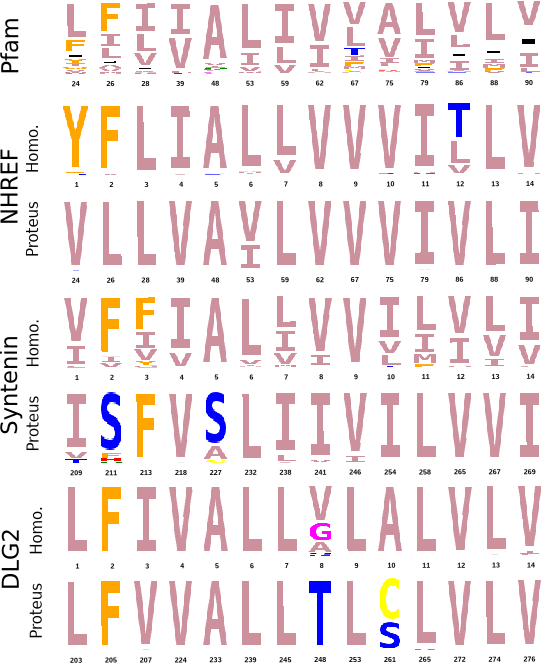
\includegraphics[trim=4.5cm 3cm 5cm 1cm, clip=true,scale=1.]{figures/logo_core.pdf}
\end{center}
\caption[width=1cm]{Core logos for Tiam1 and Cask.}
\end{figure}

\begin{figure}[!h]
\begin{center}
\vspace*{-2cm}
\includegraphics[trim=4.5cm 5cm 5cm 1cm, clip=true,scale=1.]{figures/logo_surf.pdf}
\end{center}
\caption[width=1cm]{Surface logos for Tiam1.}
\end{figure}

\begin{figure}[!h]
\begin{center}
\vspace*{-1cm}
\includegraphics[trim=1cm 4.5cm 1cm 3cm, clip=true,scale=0.9]{figures/blosumA.pdf}
\end{center}
\caption[width=1cm]{Similarity scores vs.\ Pfam for hydrophobic core.}
\end{figure}


\begin{figure}[!h]
\begin{center}
\vspace*{-1cm}
\includegraphics[trim=0cm 0cm 0cm 0cm, clip=true,scale=0.9]{figures/blosumB.pdf}
\end{center}
\caption[width=1cm]{Similarity scores vs.\ Pfam for Tiam1 and Cask.}
\end{figure}


\begin{figure}[!h]
\begin{center}
\vspace*{-1cm}
\includegraphics[trim=2.5cm 7cm 1cm 4cm, clip=true,scale=0.9, angle=90.]{figures/mdruns.pdf} 
\end{center}
\caption[width=1cm]{MD simulations of selected Tiam1 designs.}
\end{figure}

\begin{figure}[!h]
\begin{center}
\vspace*{-1.5cm}
\includegraphics[trim=0.5cm 0cm 1cm 0cm, clip=true,scale=0.85, angle=90.]{figures/titrate.pdf}
\end{center}
\caption[width=1cm]{Hydrophobic titration of Tiam1.}
\end{figure}

\begin{figure}[!h]
\begin{center}
\vspace*{-1.5cm}
\includegraphics[trim=0cm 5cm 0cm 5cm, clip=true,scale=0.5]{figures/struct_QM.pdf} \\
\includegraphics[trim=1cm 0cm 1cm 0cm, clip=true,scale=0.55]{figures/logo_QM.pdf} \\
\end{center}
\caption[width=1cm]{Designing four Tiam1 specificity positions.}
\end{figure}


\end{document}
